%%
%% This is file `tikzposter-example.tex',
%% generated with the docstrip utility.
%%
%% The original source files were:
%%
%% tikzposter.dtx  (with options: `tikzposter-example.tex')
%% 
%% This is a generated file.
%% 
%% Copyright (C) 2014 by Pascal Richter, Elena Botoeva, Richard Barnard, and Dirk Surmann
%% 
%% This file may be distributed and/or modified under the
%% conditions of the LaTeX Project Public License, either
%% version 2.0 of this license or (at your option) any later
%% version. The latest version of this license is in:
%% 
%% http://www.latex-project.org/lppl.txt
%% 
%% and version 2.0 or later is part of all distributions of
%% LaTeX version 2013/12/01 or later.
%% 
 \documentclass[17pt, a0paper, landscape, margin=0mm, innermargin=15mm,
     blockverticalspace=5mm, colspace=5mm, subcolspace=8mm]{tikzposter} %Default values for poster format options.

 \tikzposterlatexaffectionproofon %shows small comment on how the poster was made at bottom of poster
\usepackage{graphicx}
\usepackage{xpatch}
\usepackage[utf8]{inputenc}
\usepackage[english]{babel}
\usepackage[space]{grffile}
\usepackage{listings}
\usepackage{wrapfig}
\usepackage{tikz}
% Commands
 \newcommand{\bs}{\textbackslash}   % backslash
 \newcommand{\cmd}[1]{{\bf \color{red}#1}}   % highlights command


 \setlength{\tabcolsep}{2em}

 % Title, Author, Institute
 \title{\parbox{0.95\linewidth}{\centering \textbf{CODE-RADE\\ a user centric code delivery system for science}}}
 \author{
     \begin{tabular}{rl}
         Sean Murray & Bruce Becker\\
     Center for High Performance Computing & CSIR, Meraka    \end{tabular}
}
\institute{Center for High Performance Computing. CSIR, Meraka}
\titlegraphic{
    \raisebox{0cm}{
\includegraphics[scale=1.5]{img/coderade.png}}
    \hspace{1cm}\raisebox{0cm}{
\includegraphics[scale=0.125]{img/chpclogo.png}}
    \hspace{65cm}%\hfill
    \hspace{1cm}\raisebox{-1cm}{
\includegraphics[scale=0.25]{img/CSIRlogo.jpg}}
    \hspace{2cm}\raisebox{0cm}{
\includegraphics[scale=1.5]{img/coderade.png}}
    %\raisebox{0cm}{
\includegraphics[scale=0.2]{img/SANCG_logoTransparent-cropped.png}}
}
 % -- PREDEFINED THEMES ---------------------- %
 % Choose LAYOUT:  Default, Basic, Rays, Simple, Envelope, Wave, Board, Autumn, Desert,
\usetheme{Rays} % Board, Simple, Wave, Rays.
\usecolorstyle[colorPalette=BrownBlueOrange]{Rays}

\defineblockstyle{BazBlock}{%
    titlewidthscale=0.8, bodywidthscale=1, titlecenter, 
    titleoffsetx=0pt, titleoffsety=0pt, bodyoffsetx=0pt, bodyoffsety=15mm,
    bodyverticalshift=15mm, roundedcorners=22, linewidth=5pt, titleinnersep=8mm,
    bodyinnersep=8mm
    }{
        \draw[rounded corners=\blockroundedcorners, inner sep=\blockbodyinnersep, line width=\blocklinewidth, color=black, top color=titlebgcolor!90, bottom color=titlebgcolor!20!white, ]
        (blockbody.south west) rectangle (blockbody.north east); %
        \ifBlockHasTitle%
        \draw[rounded corners=\blockroundedcorners, inner sep=\blocktitleinnersep, line width=\blocklinewidth, color=black, 
        top color=titlebgcolor!90, bottom color=titlebgcolor!20!white, ]
    (blocktitle.south west) rectangle (blocktitle.north east);
    \fi%    
}

\newcommand\myblock[3][BazBlock]{\useblockstyle{#1}\block{#2}{#3}\useblockstyle{Basic}}
\makeatletter
\def\TP@titlegraphictotitledistance{-5.5cm}
\settitle
{
  \centering
  \vbox
  {
    \@titlegraphic \\ [\TP@titlegraphictotitledistance] 
    \centering
    \color{titlefgcolor}
    {\bfseries \Huge \sc \fontsize{80}{120}\@title \par}
    \vspace*{1em}
    {\LARGE \@author \par}
%    \vspace*{1.2em}
%    {\LARGE \@institute}
  }
}

\begin{document}
\useblockstyle{Basic}
\maketitle[width=0.98\textwidth]

% basic structure
% Summary of arch and tech
% schematic of code-rade workflow, the actors etc.
% diagram of delivery 
     % map of whereit can be run (grid sites)
% description of repos and repo layouts.
% todo and next features

     \begin{columns}%blocks will be placed into columns
         \column{.333}
         \block[roundedcorners=40]{Introduction}{
             \textcolor{red}{\textbf CO}ntinuous Integration and \textcolor{red}{\textbf DE}livery of \textcolor{red}{\textbf R}esearch \textcolor{red}{\textbf A}pplications in a \textcolor{red}{\textbf D}istributed \textcolor{red}{\textbf E}nvironment (CODE-RADE).
             The researcher is faced with a paradox.  There is a large amount of computing resources available, and a rich, well maintained, interoperable infrastructure of services \textbf{however} getting applications onto it requires far too much effort.\\
                  \center
\includegraphics[scale=.5]{img/legoparadox.png}\\
         
             CODE-RADE solves this by lowering the barrier to entry to grid or cloud infrastructure, or a single HPC site. 
                  Application experts are then able to prove to resource providers that the application will run on the sites execution environment. 
                  It very importantly allows easy  managing the lifecycle of applications across multiple versions, architectures and configurations. 
                  This ensures that once an application is certified, its available on as many sites as possible, and verified to work.
                  This has the knock on effect of promoting collaboration between researcher, research software engineer, and infrastructure providers. 
                  The people doing the work get citeable work as a DOI is created for a verified, peer reviewed, CVMFS release that is tied the git hashes. 
         \vspace{0.5cm}\\
         CODE-RADE has 4 principles:
         \begin{itemize}
                 \item \textbf{Cross platform} : It builds and test artifacts for an arbitrary set of targets, promoting diversity in computing platforms and ensures proper optimisations and application portability 
                \item \textbf{Atomic} :
                                 There is fine grained control over dependencies, versions, and targets and relevant actions are taken on each event in the CODE-RADE cycle. \\
                                 All these events are communicated to all willing listeners via slack.
                  \item \textbf{Community} :
                      No restriction is placed on the applications that can be integrated, anyone is free contribute; applications (dev or testing), resources(human or hardware), code review, etc. 
                  \item \textbf{Automated} :
                      Heavy reliance on automated agents to reduce bias, lead time. Humans are removed as far as possible.
             \end{itemize}

         }
        % \note[targetoffsetx=30cm,targetoffsety=12.5cm,innersep=.4cm]{After review, DOI is issued via Zenodo}%,angle=-45,connection]{DOI via Zenodo}


         \block[roundedcorners=40]{Technology}{
             \begin{itemize}
                     \item Components
                           \begin{itemize}
                               \item Version control at Github \textcolor{blue}{github.com/SouthAfricaDigitalScience}
                               \item Continuous Integration (Jenkins and Travis) \textcolor{blue}{ci.sagrid.ac.za}
                               \item Automated Delivery from successful Jenkins build to (CVMFS) /cvmfs/code-rade.africa-grid
                               \item Waffle.io is used to coordinate all human tasks, integrating with slack, and linked to github issues.
                               \item Slack is used extensively for communication via numerous bots to notify on all steps, success/failure/progress.
                               \item Open discussions at \textcolor{blue}{discourse.sci-gaia.eu}
                           \end{itemize}
                     \item Workflow 
                         Each software package has 3 scripts.
                         \begin{itemize}
                                 \item Build : User and/or expert-defined means to produce executable applications or libraries
                                 \item Test : Infrastructure operator-defined targets provide a means to ensure viability
                                 \item Deliver : Ensure that once the tests pass, the application is available at all sites.
                         \end{itemize}
                 \item All builds are inside docker containers so a user could reproduce the constant integration environment locally to test themselves, or attempt to reproduce someone
                     else's results using the exact same software.
                 \item Docker images are publicly available at quay.io/AAROC
                 \item Releases get a DOI, after review.
             \end{itemize}

         }
         \block[roundedcorners=40]{Actors}{
         Researcher
         
\includegraphics[scale=0.05]{img/labtocat.png}
         Research Software Engineer
         
\includegraphics[scale=0.05]{img/baracktocat.jpg}
         Infrastructure operations
         
\includegraphics[scale=0.05]{img/octotron.jpg}
         Automated Agents
         
\includegraphics[scale=0.05]{img/robotcat.png}
         }
         \column{0.333}
         \block[roundedcorners=40]{Workflow}{
             % 3 scripts build, check, deploy 
             % github pull request triggers a build for all versions of that application.
             % if it fails a github issue is instantiated for each version being built.
             % if it complete to deploy script, then its shipped to cvmfs.
             % each step is relayed to a slack channel to its specific channel or to generic code-rade channel for deployment.
             % operators get to review and if all happy a doi is issued against the version.
             
           \center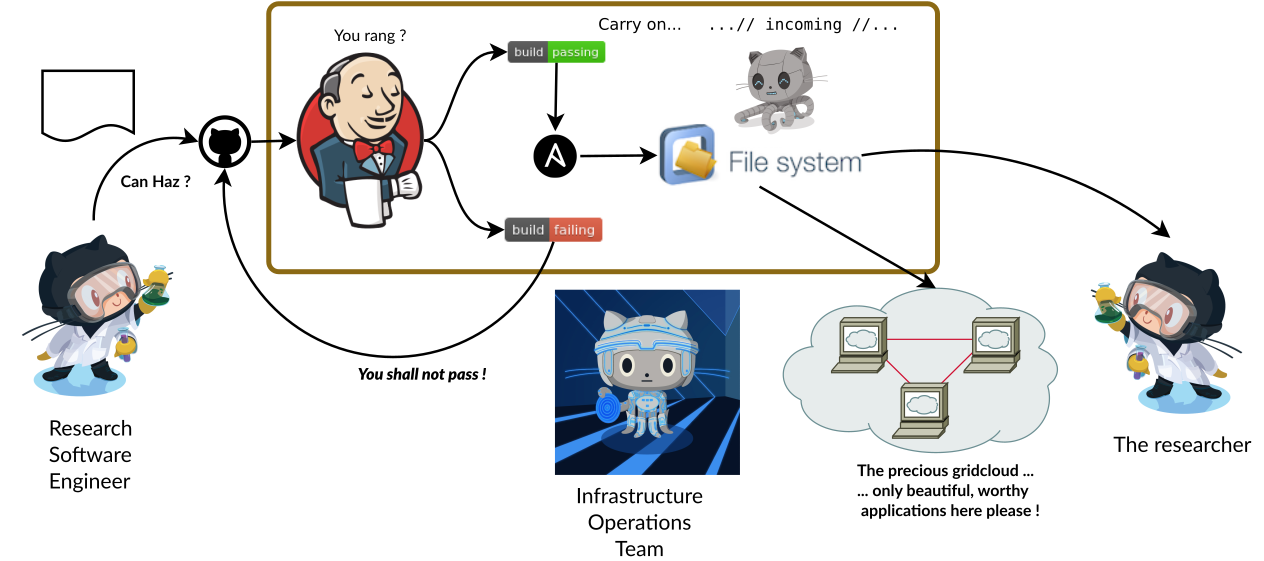
\includegraphics[scale=0.8]{img/code-rade-jenkins-magic.png}
         }
         \block[roundedcorners=40]{Deployment}{
             
           \center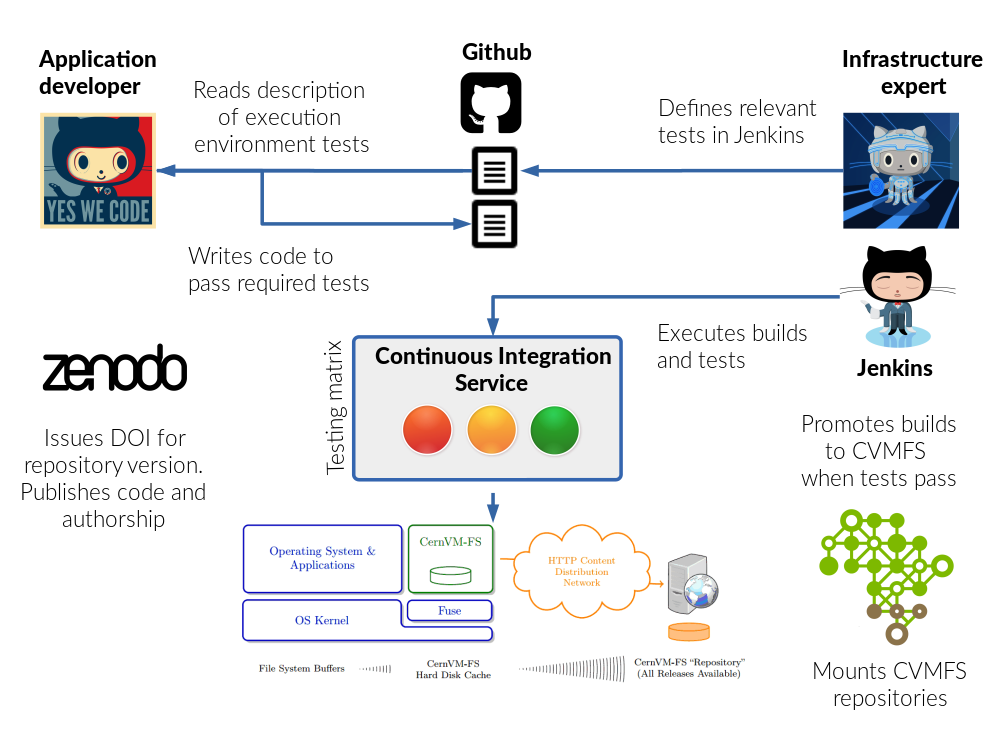
\includegraphics[scale=0.75]{img/Jenkinsworkflowschematic.png}
         }
         %      \note[targetoffsetx=30cm, targetoffsety=5cm,rotate=1,angle=270,radius=8cm,width=.15\textwidth,innersep=.4cm]{                                                                     
         %                At this point the hash and cvmfs release\\
         %                are packaged into a DOI and the pull requesters are listed as authors.                                                                                             
         %                         } 
%         \begin{subcolumns}
%         \subcolumn{0.5}
         \block[roundedcorners=40]{Architecture}{
             We build the full stack assuming nothing but the base operating system, similar to many hpc sites. We are therefore not dependent on anything local but an operational operating system and our cvmfs mount.
             \begin{itemize}
                 \item One can add as many target configurations to the build matrix as can be reliably simulated.
                 \item Currently we have defined three axes :
                 \begin{itemize}
                    \item Architecture x86\_64, ARM.
                    \item Operating System CentOS 6,7  Ubuntu 14.04 16.10
                    \item Site specific - an axis encapsulating the special nature of a site, its interconnects, compiler, local libraries, and a catch all option of generic.
                 \end{itemize} 
                     Each application is built for a combination of these dimensions, typically 1x1x4
                     With different version of complier, mpi implementations, python versions the matrix of builds and grow rapidly. 
                     For example NumPy has:\\
                     1(ARCH)x1(SITE)x4(OS)x4(PYTHON\_VERSION)x3(GCC\_VERSION)x4(NUMPY\_VERSION)=192
             \end{itemize}
        }
 %            \subcolumn{0.5}
%         \block[roundedcorners=40]{Dependency graph}{
%             \includegraphics[scale=0.2]{img/code-rade-graph.png}
%         }

         \column{.333}
         \block[roundedcorners=40]{Where can all this can run}{
             University of Free State, University of Cape Town, University of Witwatersrand, Center for High Performance Computing,
             University of Johannesburg, Moroccan National Grid, Algerian Regional Network, Zewail City of Science and Technology Egypt, and anywhere
             else prepared to mount the cvmfs repository. We are also integrated into EGI, via AfricaArabia NGI.
             \center{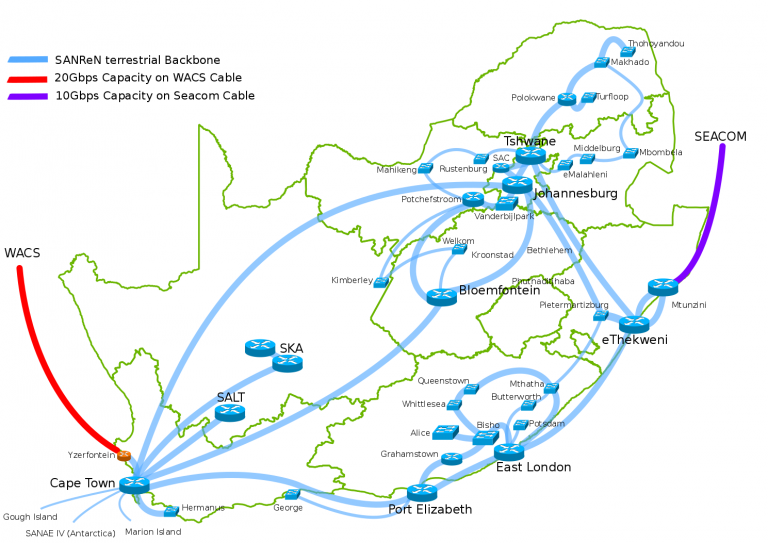
\includegraphics[scale=0.8]{img/SANReN_2016.png}
             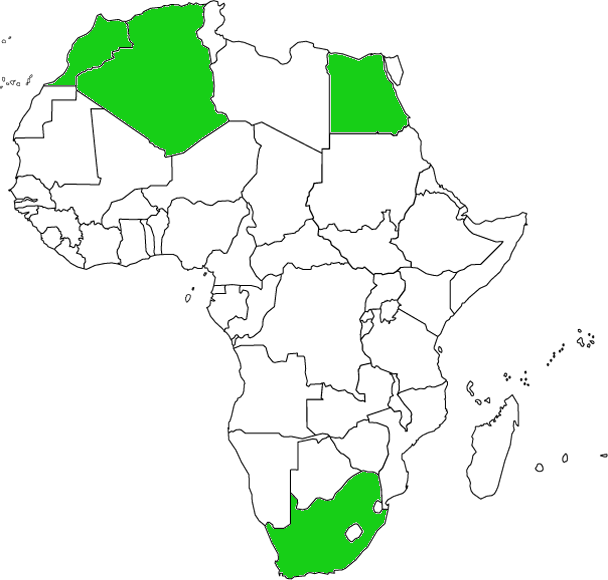
\includegraphics[scale=0.6]{img/africa-working.png}}
         }
%         \block[roundedcorners=40]{Configuration matrix}{
%             each os , each arch, each version of dependencies.
%        }
  %       \end{subcolumns}
   %  \end{columns}

     % map of whereit can be run (grid sites)
% description of repos and repo layouts.
% todo and next features

     %\begin{columns}%blocks will be placed into columns

         \block[roundedcorners=40]{Repositories}{
             Numerous pieces of software have been incorporated. The versions are very much dependent on what people want to run. We cover all fields from bioinformatics, astronomy, physics, 
             \begin{itemize}
                 \item base software from readline, zlib, pcre.
                     \item languages/compilers : python gcc 4.9.4 5.4 6.3
                         \item infrastructure : openpbs, torque.
                 \item hep : root 5.34 6.08 6.10, fastjet, geant4 9 10.1 10.3, pythia 6 8, Fermionic Molecular Dynamics, herwig, hepmc.
                 \item bioinformatics : clustal-omega  hmmer  oases  velvet  
                 \item chemistry : autodocksuite  gromacs  quantum-espresso
             \end{itemize}
             The full listing is available at both www.africa-grid.org and ci.sagrid.ac.za
        }
%         \block[roundedcorners=40]{Repository Layout}{
%             \small\lstinputlisting{examplemodule}
%         }
%         \block[roundedcorners=40]{Fermionic Molecular Dynamics}{
%               \begin{itemize}
%                   \item \textbf{Problem Area} Nuclear physics
%                   \item \textbf{Integration Time} 21 hours no prior experience
%                       \begin{itemize}
%                               \item github.com/SouthAfricaDigitalScience/FMD-codes-from-T.Neff-/
%                                   \item ci.sagrid.ac.za/view/All/job/Fermionic-Molecular-Dynamics-deploy
%                       \end{itemize}
%               \end{itemize}
%         }
         \block[roundedcorners=40]{Reproducibility}{
            \begin{itemize}
                 \item Reproducing scientific results. \\
                         One should be able reproduce \textbf{exact} workflow with the \textbf{exact expression} of the application
                         The entire repository history is kept, allowing one to relate \textbf{each successful build} to a CVMFS repository version.
                 \item Reproducing the executable application.\\
                         The \textbf{expression} of the application should be reproducible by different build systems
                          The means for expressing the application should be citeable. We this via Zenodo.
             \end{itemize}
        }
    
         \block[roundedcorners=40]{Summary and Future}{
             Making the best use of computational resources comes down to applications. We have built a cross-platform, automated system for integration and delivery of applications that :
             \begin{itemize}
                 \item Deliver functional, tested, reproducible software to a site
                 \item Recognise and reward the work of research software engineers.
                 \item Depends on only an operating system and cvmfs installed.
             \end{itemize}
             Looking forward we would like to simplify the overheads in defining new jobs and versions of software, and provide more varied architecture vectors, thereby expanding where it can run. 
        }
     \end{columns}
    \begin{columns}
    % \vspace{2cm}
        \column{0.75}
     \block[roundedcorners=40]{Acknowledgements}{%\vspace{2em}
     %\block[titleoffsety=-1cm,bodyoffsety=-1cm]{Sample document}{\vspace{2em}
        \raisebox{30cm}{
\includegraphics[scale=0.1]{img/UCTlogo.png}}
        \hspace{5cm}\raisebox{30cm}{
\includegraphics[scale=0.18]{img/UFSLogo.jpg}}
%    \raisebox{0cm}{
\includegraphics[scale=1.5]{img/coderade.png}}
        \hspace{5cm}\raisebox{31cm}{
\includegraphics[scale=0.2]{img/CSIRlogo.jpg}}
        \hspace{5cm}\raisebox{30cm}{
\includegraphics[scale=0.2]{img/SANCG_logoTransparent-cropped.png}}
        \hspace{5cm}\raisebox{32cm}{
\includegraphics[scale=0.1]{img/chpclogo.png}}
        \hspace{5cm}\raisebox{32cm}{
\includegraphics[scale=1.2]{img/magrid.png}}
        \hspace{5cm}\raisebox{32cm}{
\includegraphics[scale=1.2]{img/arn.png}}
        \hspace{5cm}\raisebox{32cm}{
\includegraphics[scale=1.2]{img/zc.png}}
   %
\includegraphics[scale=0.1]{img/UCTlogo.png}  
%   \raisebox{0cm}{
\includegraphics[scale=0.12]{img/UFSLogo.jpg}}
%%    \raisebox{0cm}{
\includegraphics[scale=1.5]{img/coderade.png}}
%    \raisebox{-1cm}{
\includegraphics[scale=0.25]{img/CSIRlogo.jpg}}
%    \raisebox{0cm}{
\includegraphics[scale=0.2]{img/SANCG_logoTransparent-cropped.png}}
%    \raisebox{0cm}{
\includegraphics[scale=0.15]{img/chpclogo.png}}
%    \raisebox{0cm}{
\includegraphics[scale=1.52]{img/magrid.png}}
%    \raisebox{0cm}{
\includegraphics[scale=1.52]{img/arn.png}}
%    \raisebox{0cm}{
\includegraphics[scale=1.52]{img/zc.png}}
%   \center Feedback and discussion at discourse.sci-gaia.eu
 %  \begin{flushright}
\includegraphics[scale=0.25]{img/SANCG_logoTransparent-cropped.png}\end{flushright}
     }
        \column{0.25}
     \block[roundedcorners=40]{Further Information}{%\vspace{2em}
         \centering{
        \textcolor{blue}{\textbf{github.com/AAROC/CODE-RADE}}\\
        africa-arabia-roc.slack.com\\
        Sean Murray at murrays@cern.ch\\
        Bruce Becker at bbecker@csir.co.za

    }}

    \end{columns}
 \end{document}




\endinput
%%

%% End of file `tikzposter-example.tex'.
